
\subsection{Block analysis}


\begin{figure}[t]
    \centering
    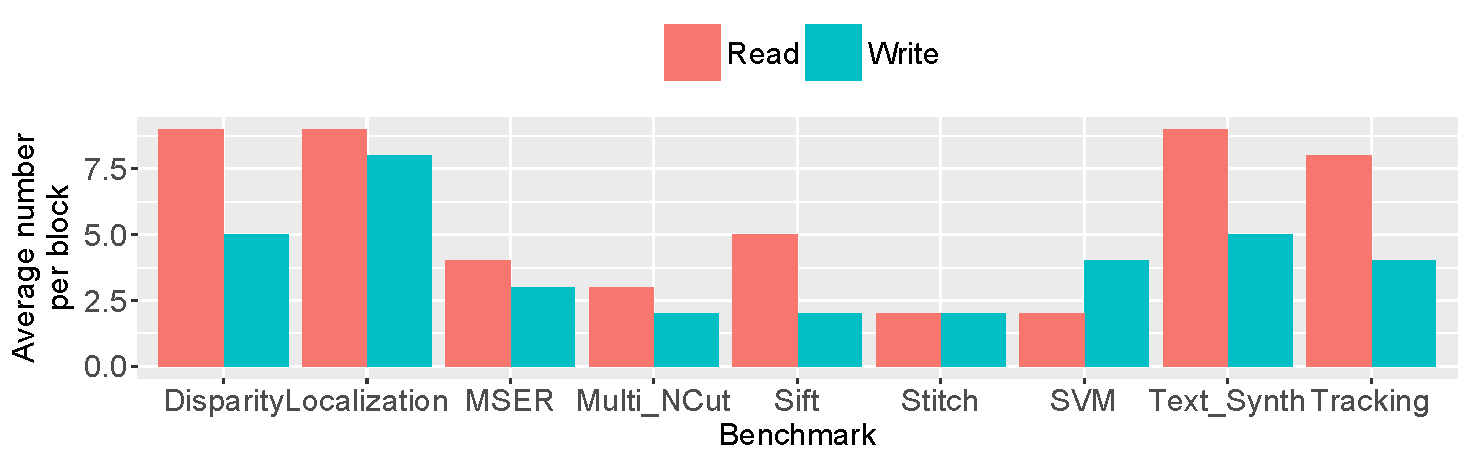
\includegraphics[width=1\textwidth]{chapter3/graphics/averageRegRead.pdf}

    \caption{Average number of register reads and writes per EDGE block.}
    \label{fig:edge_reg_read}
	\vspace{1em}
\end{figure}

One of the defining factors of the block based D-VTAGE predictor is that a single prediction fetches a fixed set of values rather than a single prediction.
Due to the fact that the block size is fixed ahead of time~\cite{peraisBeBop2015}, determining the correct size is important.
Having a block with many values means that the D-VTAGE predictor can predict a higher amount of register reads in the EDGE block, however this comes at the expense of having less blocks in the predictor tables.
On the other hand, a small block size allows to have multiple blocks stored at a time but means that not all instructions can have their values predicted in the EDGE block.

In this chapter, the value predictor can only predict register reads rather than predicting values for any instruction.
This is due to the fact that register reads create data dependencies amongst blocks, as discussed in Section~\ref{chp3:sec:val}.
Focussing only on register reads also reduces the the block size requirements as there is often only a few reads in an EDGE block.
To determine the size, all the EDGE blocks of the SD-VBS benchmarks are anaylsed to find out the what the average register read and write count is per block.
The writes are tracked as it provides information on the potential amount of register dependencies found in each of the applications.

Figure~\ref{fig:edge_reg_read} shows the average number of register read and writes for each of the benchmarks.
On average, there are 5 register reads and 3 register writes per block.
Whilst \bm{Disparity} \bm{Localization}, \bm{Texture\_Synthesis} and \bm{Tracking} have higher register read counts than the average, most of them only have 5 writes per block.
This potentially means that having a D-VTAGE block size of 5 would capture all dependencies.
However this would require either compiler support to mark register reads that potentially need value prediction, or have hardware to detect register reads that lead to data-dependencies to figure out which register read instructions should be in the predictor; this work is left for future endeavours.
Therefore, to ensure that most blocks have all their register reads captured, a block size of at least 8 is required.
More details on how block size affects performance of the predictor can be found later on in this section.

\subsubsection{Block variation analysis}

\begin{figure}[t]
    \centering
    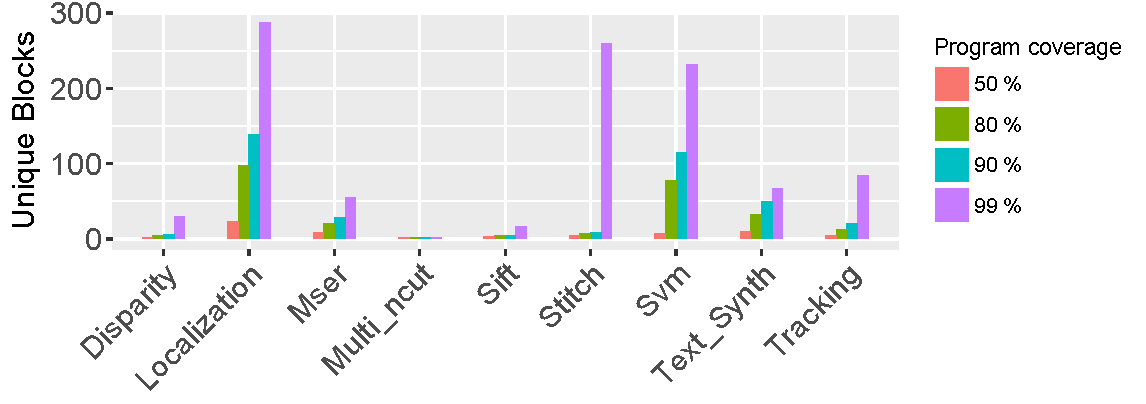
\includegraphics[width=1\textwidth]{chapter3/graphics/unique_blocks.pdf}

    \caption{Number of unique blocks comprising different percentages of the total execution (in blocks) of each of the benchmarks.}
    \label{fig:totblock}
	\vspace{1em}
\end{figure}

One method of understanding how the block based D-VTAGE predictor will perform is to study the number of unique blocks found in each of the benchmarks.
Benchmarks that feature a smaller number of unique blocks can potentially benefit more from value prediction as the predictor cannot hold many blocks at a time.
Reporting all unique blocks executed is not a proper evaluation of the variety of blocks found in the benchmark, as some will most certainly be executed more times than other.
To account for this, blocks are sorted by number of occurences in descending order, and then added to the unique block counter as long the number of occurences of visited blocks is under a percentage of total number of blocks executed.

Figure~\ref{fig:totblock} shows the number of unique blocks found in each benchmark that account for 50,80,90 and 99\% of the total number of executed blocks.
As can be seen, applications \bm{Disparity}, \bm{Multi\_NCut} and \bm{Sift} \bm{Stitch} and \bm{Tracking} execute less than 50 unique blocks during 90\% of its total execution.
This is promising as it means that there is a high chance that the predictor requires less entries to capture all possible blocks in the application.
On the other hand, \bm{Localization}, and \bm{SVM} execute over 100 blocks throughout 90\% of their execution, twice as many as the previously mentioned benchmarks.
For these applications, it migth be harder to predict values as new blocks may overwrite entries in the predictor.


\subsection{Setup}
This section demonstrates how the block based D-VTAGE value predictor improves the performance of core composition using the round-robin fetch scheme (RRF).
Serial fetch is not explored as the previous section showed that when considering value prediction, RRF always provides the best results.
The results reported in this section represent the culmination of hardware modifications for core composition discussed in this chapter.

The objective of this section is to demonstrate that a state of the art value predictor, paired with a new fetching scheme, can be used to improve the performance of large core compositions, and to show the difference between a real predictor and the perfect predictor.
The D-VTAGE size configuration can be found in Table~\ref{tab:vtage-conf}.
The Last-Value Table shares the same number of values as the Base Entry and uses a 5-bit tag.
Each tagged entry has a tag of varying size (first table is 12 bits, second 13 bits so on and so forth).
The total number of values for the D-VTAGE predictor is taken from Perais et al's original paper which introduced the predictor~\cite{peraisBeBop2015}.\
The adpoted size for this chapter is the medium predictor as it provides a good compromise between performance and memory footprint.
It is important to note that in this context, the values represent single entries in the table, they can be grouped up into any number of blocks.

The blocks in the speculative window represents the total number of in-flight blocks that can be handled by the speculative window.
As each core can only have up to four blocks live, the speculative window is set to have four block.
For the size of the stride, 64 bit values are used throughout the experiments to maximise the reach of the predictor.
However, different stride sizes are considered: the simulator tracks the size of the strides used in valid predictions to detect how small the strides can be made for each of the benchmarks.
The analysis of the stride size is discussed later on in this section.

Two features of the predictor can be modified: the number of values per entry and at what confidence a prediction is used.
Modifying the required confidence explores the trade-off beteween high coverage and low misprediction.
The original D-VTAGE uses Forward Probabilistic Counters (FPC)~\cite{riley2006fpc} to increment the confidence, and only used predictions once the counter was set to 7.
To briefly summarise FPC: when a value is correctly predicted, its confidence is incremented based on a probability, rather than always incrementing the counter by one.
This section explores two counter scenarios: using a prediction when the confidence is set to 4 (without FPC), and using confidence when the counter is set to 7 (with FPC).
The confidence of 4 is chosen as it allows for very fast deployment of predictions, whilst still ensuring that the values have been trained at least a few times.
The FPC vector used in this Chapter is the same as the one in Perais et al.'s work $\{1,\frac{1}{16},\frac{1}{16},\frac{1}{16},\frac{1}{16},\frac{1}{16},\frac{1}{32},\frac{1}{32}\}$.
This confidence rate ensured that the predictor had an accuracy of over 99\%, but at the expense of a low coverage, 20\% on average~\cite{peraisBeBop2015}.


\begin{table}[t]
  \small
  \centering
 \begin{tabular} {| l | l | l |}
 \hline
	\#Base Entry. & \#Tagged & \#Block in Spec Window\\ \hline
	1536 & $6\times1536$ & 4 \\ \hline
	\end{tabular}
  \caption{D-VTAGE table configuration.}\label{tab:vtage-conf}
\end{table}

\begin{table}[t]
\small
\centering
\begin{tabular}{p{5.2cm} p{1.8cm}}
\toprule
\textbf{Parameter} & \textbf{Values} \\ \midrule
\# of values per entry & 8, 16\\
Confidence Value & 4 or 7 with FPC \\ \bottomrule
\end{tabular}
\caption{Configurable parameters for D-VTAGE}\label{tab:vtage-params}
\vspace{1em}
\end{table}

Table~\ref{tab:vtage-params} shows the possible values that can be taken for the two parameters.
Whilst this section previously showed that most applications only have 5 reads per block, this section explores block sizes of 8 and 16 to ensure that all register reads are potentially covered. 
Once again, all benchmarks are executed using a 16 core composition.

\subsection{Results}

\subsubsection{Performance}

\begin{figure}[t]
    \centering
    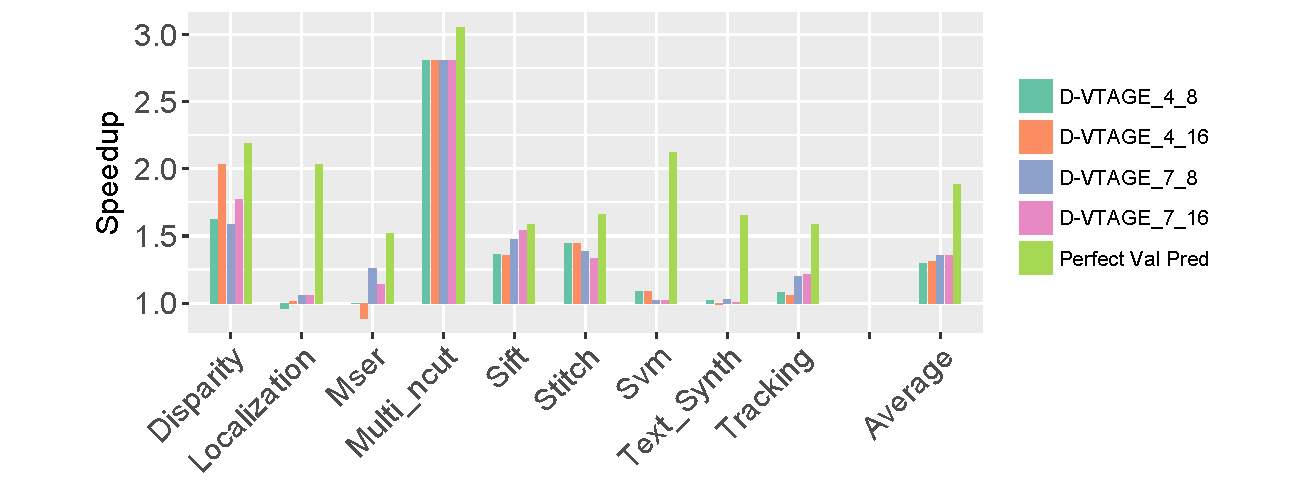
\includegraphics[width=1\textwidth]{chapter3/graphics/vtage_speed2.pdf}
    \caption{Comparing the performance of the standard fetching scheme to the new fetching scheme, with and without perfect value prediction. Higher is better.}
    \label{fig:vtage_perf}
	\vspace{1em}
\end{figure}

Figure~\ref{fig:vtage_perf} reports the speedup obtained with the different configurations of the D-VTAGE predictor with RRF.
The baseline is a 16 core composition that uses the serial fetching (SF) scheme without any value prediction and using perfect branch prediction.
The lack of value prediction and use of serial fetching represents the current implementation of core composition.
To better understand the performance of the predictors, each configuration is compared to the perfect predictor, which can predict every register value at any instance.
Throughout this section, the configurations of D-VTAGE are labelled: \textbf{D-VTAGE\_\textit{Confidence}\_\textit{BlockSize}}.

On average, using a D-VTAGE value predictor with the Round Robin Fetch scheme results in an average speedup of 1.32x.
When comparing the performance between the different configurations, the main observation is that using a higher confidence results in better performance, however slight, 1.35x for D-VTAGE\_7\_16 compared to 1.31x for D-VTAGE\_4\_16.
However, for the benchmark \bm{Disparity} using a higher confidence leads to less of a performance increase 1.75x speedup compared to 2.0x for a confidence counter of 4.
This is due to the fact that \bm{Disparity} is composed of loops with highly predictable values, and thus deploying predictions faster results in better performance improvements without risking a higher misprediction rate.
On the other hand, \bm{Localization} and \bm{MSER} performs worse with a lower confidence counter, and result in a slowdown.
Benchmarks \bm{Sift} and \bm{Tracking} perform better with a higher confidence, but the results of using a 4 bit counter never negatively impact performance.

When it comes to the size of a block, often the 16 values does not lead to better performance than 8 values but stays on par with it.
The only noticeable difference is with \bm{MSER} where the smaller block performs better.
As previously mentioned, a lower number of values per block allows the predictor to capture a higher variety of executed blocks.
Figure~\ref{fig:totblock} shows that \bm{MSER} has at least 50 different blocks throughout 99\% of its execution, and Figure~\ref{fig:edge_reg_read} shows that the benchmark has, on average, only 3 register reads per block.
Therefore, for \bm{MSER}, a predictor with less values per entry can capture more of the variation.
On the other hand, for \bm{Disparity}, 16 values per entry is required to get the best performance.
This once again corroborates with the information from Figures~\ref{fig:totblock} and ~\ref{fig:edge_reg_read}.
\bm{Disparity} has a higher average of reads per block, but features a very low number of unique blocks.
Therefore having a larger entry in the table captures more values that can be predicted, but does not suffer from having entries being replaced by new blocks.

Comparing the performance of the different D-VTAGE configurations to the perfect value predictor, it is apparent that most benchmarks do not achieving their maximum potential as the perfect predictor results in an average speedup of 1.88x compared to 1.32x of D-VTAGE.
However, benchmarks \bm{Disparity} and \bm{Multi\_NCut} show how value prediction paired with RRF is a promising lead for improving the performance of core composition.

\subsubsection{Coverage and Accuracy}
To better understand the performance of the different D-VTAGE configurations, the predictors' coverage and misprediction rates are recorded.
Since EDGE is a block based architecture, it is important to study the coverage and accuracy on both a per-instruction level and per-block level.
This is due to the fact that a single read misprediction leads to flushing the block and all younger blocks in the chain.
Thus whilst the misprediction rate for predicted instructions may be low, it can have a large impact as up to 64 blocks may be in flight, and may all need to be flushed.
Also a single accurate register prediction may not necessarily improve performance as other un-predicted registers in the block may be data-dependent with other blocks, reducing ILP.

\begin{figure}[t]
    \centering
    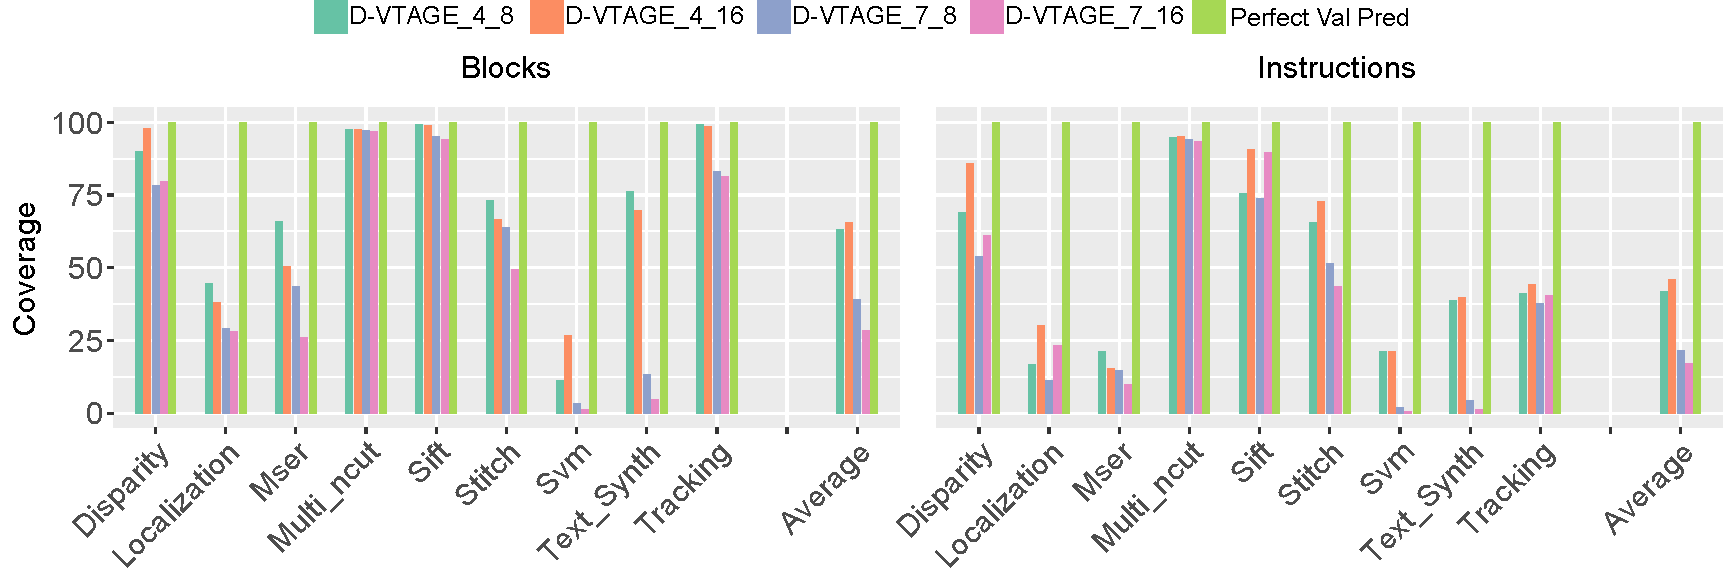
\includegraphics[width=1\textwidth]{chapter3/graphics/coverageFull.pdf}
    \caption{Prediction coverage at a block and instruction level. Higher is better}
    \label{fig:vtag_cov_block}
	\vspace{1em}
\end{figure}

Before looking at the accuracy of the predictors, it's important to study the coverage as it gives an overall view of how active the value predictor is during the execution of a program.
In this chapter, only blocks that are committed count towards the predicted blocks, as flushes caused by LSQ violations, for example, may artificially inflate the coverage count, as a flushed block may have issued a prediction.
Figure~\ref{fig:vtag_cov_block} displays the number of blocks which have at least one prediction, relative to the total number of committed blocks and the number of predicted register reads relative to the total executed register reads.
The figure shows similar patterns for both coverages: the predictors with lower confidence counters have a higher coverage, 65\% compared to 31\% for the high confidence counter.
This is normal, as lower confidence causes predictions to be used with less training, and thus increases the number of predictions used during the execution of the program.

Whilst the block coverage is high, the coverage for registers reveals that not all registers are being predicted.
Once again, lower confidence equates to higher coverage, however this time it's 30\% for a confidence of 4 and under 25\% for a confidence of 7.
The register coverage for a confidence of 7 is in line with the coverage reported in Perais. et al's work ~\cite{peraisBeBop2015, peraisVTAGE2014} if not slightly higher.
The coverage may be slightly higher due to the fact that the values being predicted are often either loop increments or memory increments which can easily be predicted.

The register coverage helps explain why the high block coverage does not lead to better performance: whilst most blocks may have a valid prediction, some of the register reads cannot be predicted.
This may be due to data being carried over which is unpredictable; for instance a loop which sums all values of an array into a single integer will pass that integer via a register.
This register will cause a data dependency between loop iterations and cannot be predicted unless the values in the array are highly predictable.
Even if the register coverage is low, any correct prediction can help improve performance as blocks can use the values as they wait to receive the real value from the NoC.

\bm{Localization}, \bm{MSER}, \bm{SVM} and \bm{Texture\_Synthesis} often have much lower coverage than the rest of the programs.
Recalling Figure~\ref{fig:totblock} which shows the number of unique blocks executed throughout the programs, these benchmarks had a higher count of unique blocks.
This explains why the coverage will be lower: there's a higher chance of encountering a new block than executing a known one.
As blocks require multiple executions to train the predictor (if the values in the register are indeed predictable), than the higher diversity of blocks makes it harder.
Thus, these benchmarks will naturally have a harder time to benefit from value prediction.

Figure~\ref{fig:vtag_cov_block} shows that a lower confidence allows for higher coverage, yet the speedups seen in Figure~\ref{fig:vtage_perf} indicate that a higher confidence leads to better performance.
Intuitively, this must mean that the lower confidence leads to a higher misprediction rate.
To confirm this, Figure~\ref{fig:vtag_accuracy_block} presents the prediction accuracy rate for each benchmark at a per-block and per-instruction base respectively.
The D-VTAGE predictor maintains a 99\% accuracy, whether at the block level or instruction level.
However, for \bm{Localization}, \bm{MSER}, \bm{SVM}, \bm{Texture\_Synthesis} and \bm{Tracking}, the block level accuracy for a confidence of 4 is under 98\%, and even down to 93\% for \bm{MSER}.
The effect of a value misprediction is similar to a branch misprediction: it causes a flush of all blocks younger than the block with the incorrect misprediction.
Just like branch prediction, large core compositions are very sensitive to mispredictions, thus an accuracy rate of 93\% will impact performance if the blocks are small.
This explains why the low confidence counter sometimes performs worse than the higher confidence as it mispredicts more often.

\begin{figure}[t]
    \centering
    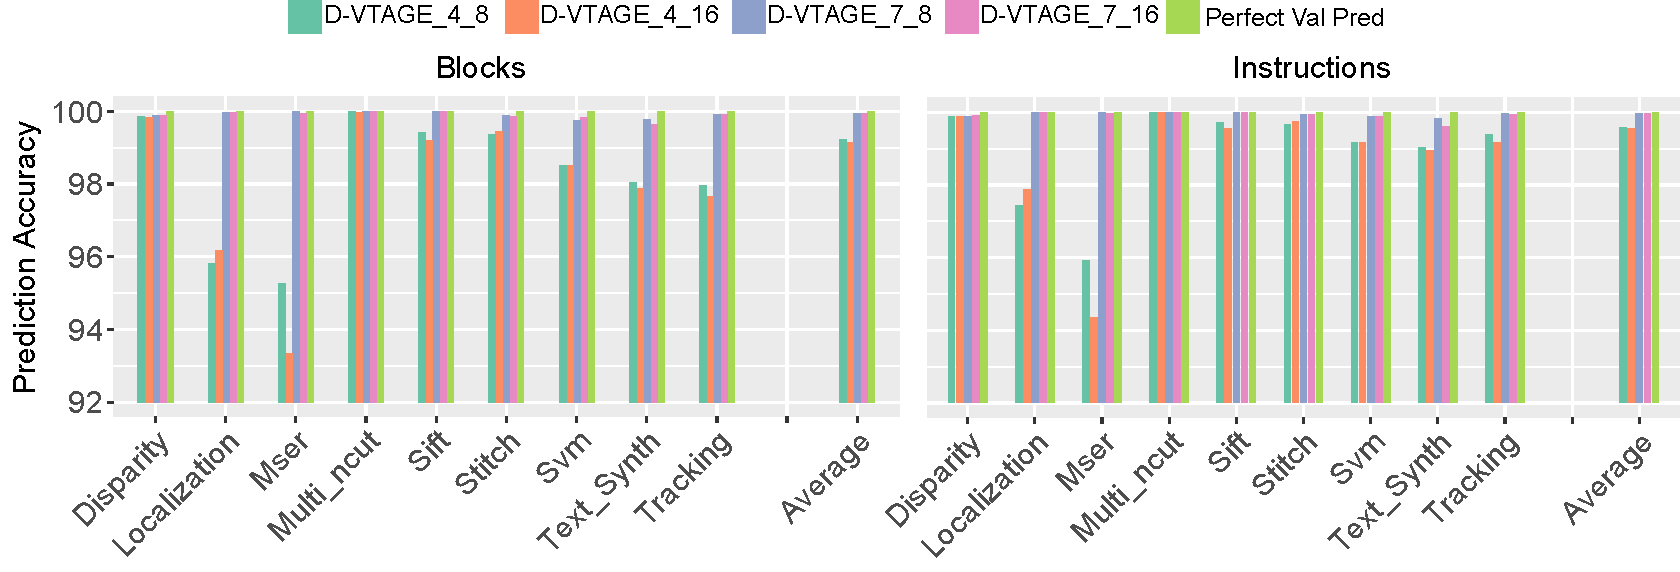
\includegraphics[width=1\textwidth]{chapter3/graphics/predAcc.pdf}
    \caption{Accuracy of the different D-VTAGE predictors at a block and instruction level. Higher is better.}
    \label{fig:vtag_accuracy_block}
	\vspace{1em}
\end{figure}
\subsubsection{Size of stride}

\begin{figure}[t]
    \centering
    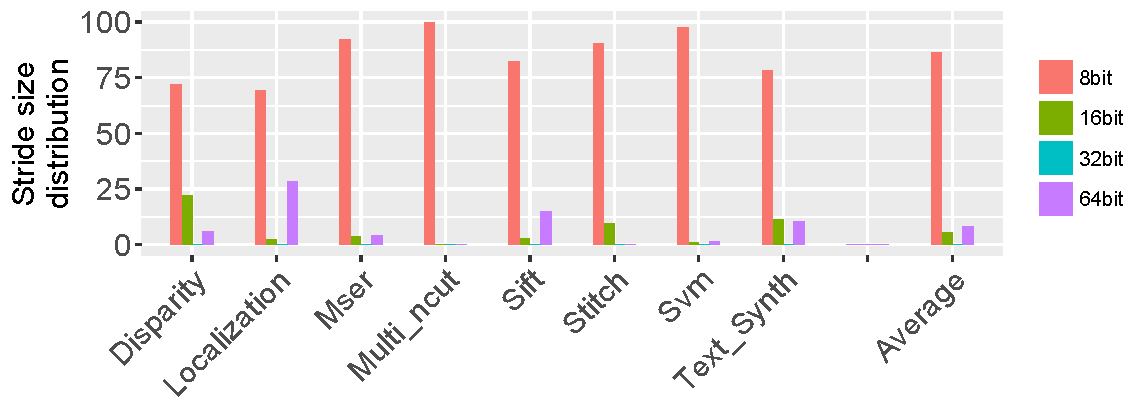
\includegraphics[width=1\textwidth]{chapter3/graphics/strides.pdf}
    \caption{Distribution of the size of strides for each benchmark.}
    \label{fig:strides}
	\vspace{1em}
\end{figure}

Whilst 64 bit strides are used throughout the experiments to capture all the potential performance, 64 bits per entries may not be necessary.
Figure~\ref{fig:strides} shows the average number of valid predictions whose strides could fit in either an 8, 16, 32 or 64 bit signed integer for each of the benchmarks.
The data was taken from the D-VTAGE configuration that led to the highest performance overall for each of the benchmarks.
In Perais' et al'.s work they recommend that a medium-sized D-VTAGE predictor use 8-bit strides.
Overall, Figure~\ref{fig:strides} shows that using 8 bit strides should be sufficient for most benchmarks, however \bm{Disparity}, one of the benchmarks which benefits most from value prediction, would lose almost 25\% of its coverage.
Therefore, for these set of applications, a stride of at least 16 bits is necessary, as it captures 91\% of the total strides found in all the benchmarks.

\subsection{Putting it all together}
This section has demonstrated that a real value predictor can sometimes perform as well as a perfect predictor, resulting in a speedup of up to 2.7x for \bm{MSER} and 2x \bm{Disparity}, when paired with the round robin fetching scheme.
The section also showed that whilst a lower confidence rate does increase the coverage, it does lead to a higher misprediction.
As core composition is sensitive to any kind of misprediction that causes a flush, the predictor with confidence value 4 performs less well than confidence value 7 with FPC.
Finally, the analysis of stride size shows that for this set of benchmarks, a 16 bit stride is sufficient to capture 91\% of the strides for the benchmarks.
Using this information, a recommended D-VTAGE configuration for the dynamic multicore processor would take up 39kB of memory, which is slightly larger than an L1 cache.
